\section{Обзор архитектуры}

\section{Эхехех}

Табличка \ref{tab:features_and_dim_reduction}.

\begin{table}[ht]
\newrobustcmd{\B}{\bfseries}
\renewcommand\tabularxcolumn[1]{m{#1}}
\begin{tabularx}{1\textwidth}
{ 
  | >{\raggedright\arraybackslash}X 
  | >{\centering\arraybackslash}X
  | >{\centering\arraybackslash}X |}
    \hline
        & Блабла \\ \hline\hline
        16 ааа                                   &    0.253 &    0.61  \\ \hline
        100 ббб                                  & \B 0.326 & \B 0.742 \\ \hline\hline
        хахахаха             &    0.380 &    0.826 \\ \hline
        азазаззаза                                            & \B 0.454 & \B 0.926 \\ \hline
        ляляляля       &    0.452 &    0.916 \\ \hline
\end{tabularx}
\captionof{table}{Название табличка  \mbox{какая то еще штука} }
\label{tab:features_and_dim_reduction}
\end{table}

\section{аааа}

Рисуночек.

\begin{figure}[ht]
    \centering
    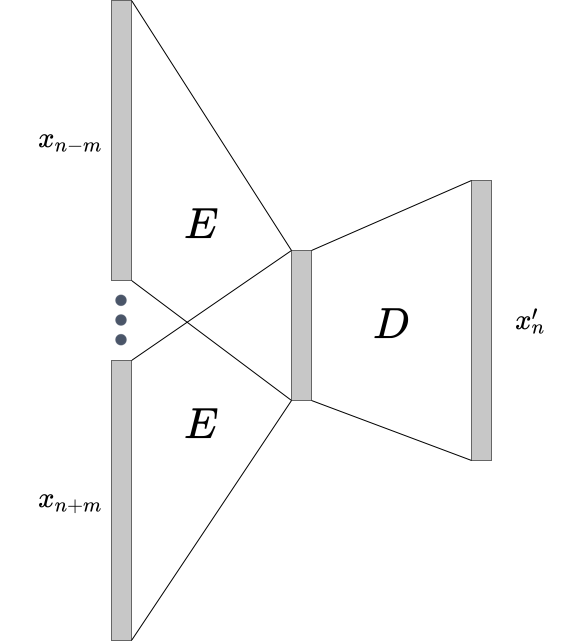
\includegraphics[width=0.6\linewidth]{imgs/CBoW.png}
    \caption{\centeringАрхитектура CBoW. $E$-- энкодер. $D$-- декодер. $x$-- one-hot векторы слов, $m$-- размер контекста}
    \label{fig:CBoW}
\end{figure}

Еще рисуночек.

\begin{figure}[ht]
    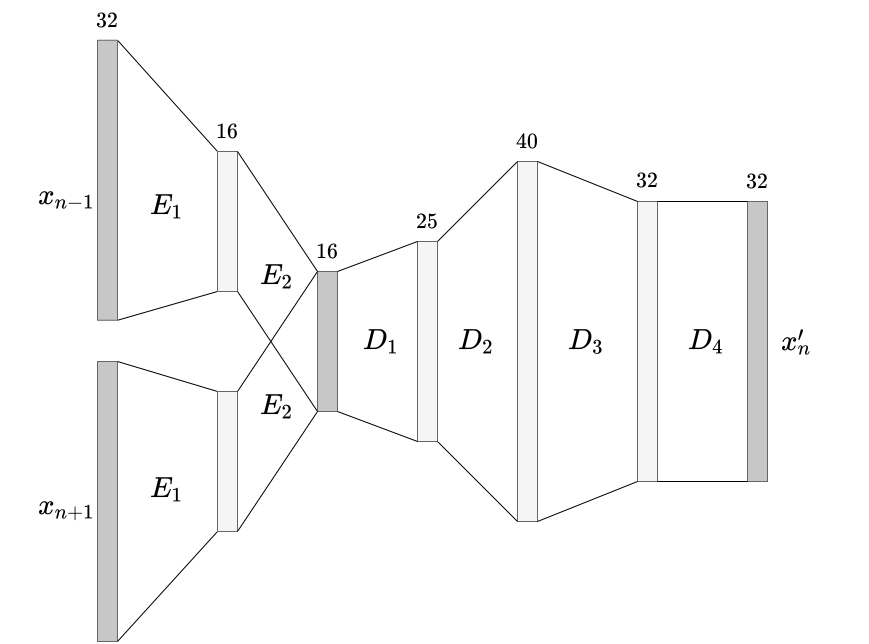
\includegraphics[width=\linewidth]{imgs/CBoS.png}
    \caption{\centeringАрхитектура CBoS. $E$-- полносвязные слои энкодера, $D$-- полносвязные слои декодера, $x$-- векторы признаков.}
    \label{fig:CBoS}
\end{figure}

\begin{table}[ht]
\renewcommand\tabularxcolumn[1]{m{#1}}
\newrobustcmd{\B}{\bfseries}
\begin{tabularx}{1\textwidth}
{ 
  | >{\raggedright\arraybackslash}X 
  | >{\centering\arraybackslash}X
  | >{\centering\arraybackslash}X |}
    \hline
        & Adjusted rand score & Homogeneity Score \\ \hline\hline
        Исходные признаки                                       &    0.459 &    0.925 \\ \hline
        CBoS                                                    & \B 0.615 & \B 0.931 \\ \hline
        Autoencoder                                             &    0.449 &    0.922 \\ \hline
\end{tabularx}
\captionof{table}{Сравнение качества кластеризации данных алгоритмом \mbox{K-Means} на 50 классов для методов CBoS и Autoencoder с исходным пространством признаков}
\label{tab:orig_vs_cbos_vs_auto}
\end{table}


\section{Восстановление текста}
\titlespacing*{\subsection}{\parindent}{*-2}{*0}
\subsection{Восстановление знаков из классов}
\titlespacing*{\subsection}{\parindent}{*4}{*0}

\subsection{Лингвистическая модель}
\label{section: bigramm language model}

\subsection{Классификация и цикл обратной связи}

Ссылочка на секцию \ref{section: bigramm language model}.


















